%% system description: 
%% persona agent layer
%% task specific layer (e.g., for type 2 chatbot, chatbot api + eval api)

\section{System Description}
\begin{figure}
    \centering
    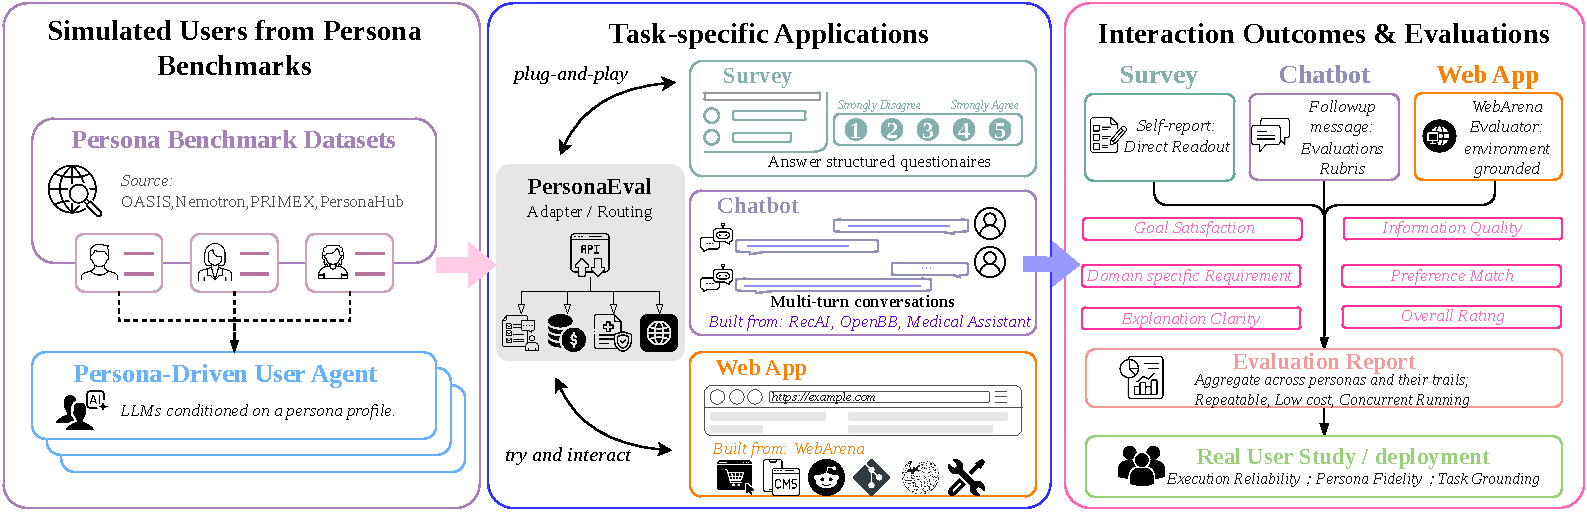
\includegraphics[width=0.98\linewidth]{figures/PersonaEval.pdf}
    \caption{
    \textbf{Overview of \method.}
    \method connects persona-driven simulated users to different types of applications through plug-and-play adapters and provides a unified workflow for collecting interaction outcomes, feedback, and evaluation reports.
    }
    \label{fig:personaeval}
\end{figure}

\method(~\autoref{fig:personaeval}) is a system for evaluating interactive applications through simulations of realistic users. Each simulation uses a simulated user with predefined persona attributes, such as background, preferences, and communication style (~\autoref{fig:within-clusters}). 
% This lets \method test how the same application is experienced by different kinds of users in a repeatable way. 
Each simulation run is executed inside a sandbox with declared resources and controlled dependencies, which provides the runtime boundary for the evaluation and keeps the persona side and the task side isolated from other applications. This is important because different applications may need different code, data, tools, browser environments, or backend services.


\paragraph{Persona API.} The persona API wraps a persona model as a simulated user. It receives the assigned persona and the task instruction, then produces the next user behavior through the interface required by the task. Depending on the application type, this behavior can be a survey response, a chat message, or a computer-use action. 
% The persona API is responsible for staying in character and acting from the assigned user's point of view.

\paragraph{Task API.} The task API packages the environment needed to test a particular application. It defines the task instruction, hosts or connects to the application under test, manages the interaction protocol, and provides the evaluation form. For example, a chatbot task connects the simulated user to a chat API, and a web task hosts a website and exposes it through a browser environment. This design lets each task define its own environment and evaluation criteria while sharing the same simulation workflow.

% \paragraph{User inferface.} The interface is organized around the same workflow. The left-hand panel is used to choose and inspect the simulated user by persona. The center panel configures the task, including the application type and the run settings. The main trace view shows the interaction as it unfolds, including survey responses, chatbot turns, or web actions. The right-hand panel summarizes the evaluation form completed by the simulated user. 
% % This layout makes each simulation reviewable from persona selection to task execution and final feedback.